% Brian Mc George - MCGBRI004
% Jacques Heunis - HNSJAC003
% Timothy Gwynn - GWNTIM001
% Due: 31-07-2015
% Stage One - Software Engineering  - CSC3003S
\documentclass[a4paper,10pt]{article}
%**************************************************************************************************
% PACKAGES
%**************************************************************************************************
\usepackage{amsmath, amsthm, amsfonts, amssymb}
\usepackage{graphicx,color}
\usepackage{bm}	
\usepackage{float}
\usepackage{caption, subcaption}
%\usepackage{vector}

%**************************************************************************************************
% DEFAULT SETTINGS
%**************************************************************************************************
\marginparwidth -20 true pt    % Width of marginal notes.
\oddsidemargin  -10 true pt       % Note that \oddsidemargin=\evensidemargin
\evensidemargin -10 true pt
\topmargin -0.5 true in        % Nominal distance from top of page to top of
\textheight 9.75 true in         % Height of text (including footnotes and figures)
\textwidth 7 true in        % Width of text line.
\parindent=10pt                  % Do not indent paragraphs
\parskip= 1 ex
\columnseprule = 0.1pt
\footskip = 30 true pt
\hoffset = -0.1 true in
\voffset = -0.1 true in
\abovedisplayskip 1 true pt
\abovedisplayshortskip 1 true pt
\topsep 0 true pt
\newcommand*\varhrulefill[1][0.4pt]{\leavevmode\leaders\hrule height#1\hfill\kern0pt}

%**************************************************************************************************
% DOCUMENT DETAILS
%**************************************************************************************************


%**************************************************************************************************
% MAIN DOCUMENT 
%**************************************************************************************************

\begin{document}
\begin{titlepage} \begin{center} 
		\textsc{\LARGE University of Cape Town}
		\\[1.5cm] \textsc{\Large Software Engineering Stage One\\CSC3003S}
		\\[0.5cm]
		\noindent\rule[0.4mm]{\textwidth}{0.1mm}
		\\[0.4cm] { \huge \bfseries Tempest Trace \\[0.4cm] }
		\noindent\rule[0.4mm]{\textwidth}{0.1mm}
		\\[1cm]
		\begin{minipage}[t]{0.4\textwidth}
		\begin{flushleft}\large \emph{Authors:}\\ Brian Mc George - MCGBRI004 \\ Jacques Heunis - HNSJAC003 \\ Timothy Gwynn - GWYTIM001\end{flushleft}
		 \end{minipage} \begin{minipage}[t]{0.4\textwidth} 
		\begin{flushright} \large \emph{Supervisor:} \\ Assoc. Prof.~Patrick Marais\\patrick@cs.uct.ac.za\end{flushright}
		\begin{flushright} \large \emph{Tutor:} \\ Codie Roelf\\Codie.Roelf@alumni.uct.ac.za\end{flushright}
		 \end{minipage} \vfill {\large \today}
		\end{center}
		\end{titlepage}
\newpage
\tableofcontents
\newpage

\section{Use Case Narratives}

\section{Analysis Class Model}
\begin{figure}[H]
	\begin{center}
		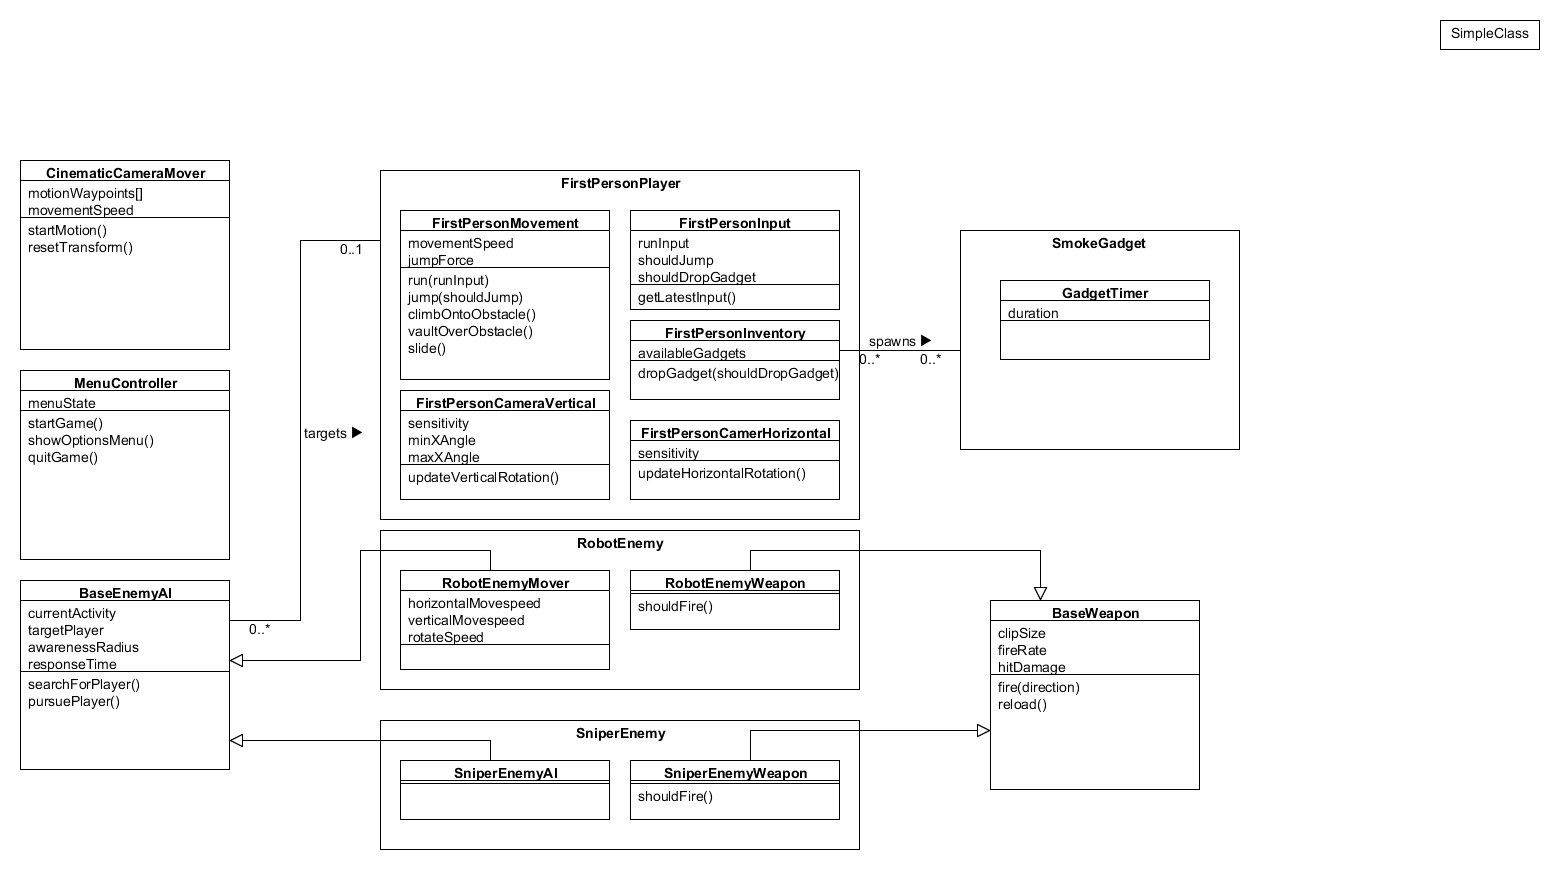
\includegraphics[scale=0.4]{images/AnalysisClassDiagram.png}
		\caption{Get analysisized!}
	\end{center}
\end{figure}
A first-draft analysis class model.

\section{State Diagrams}

\section{Project Plan}

\section{Test Plan}

\end{document}
